% Created by tikzDevice version 0.12.6 on 2025-02-05 15:21:44
% !TEX encoding = UTF-8 Unicode
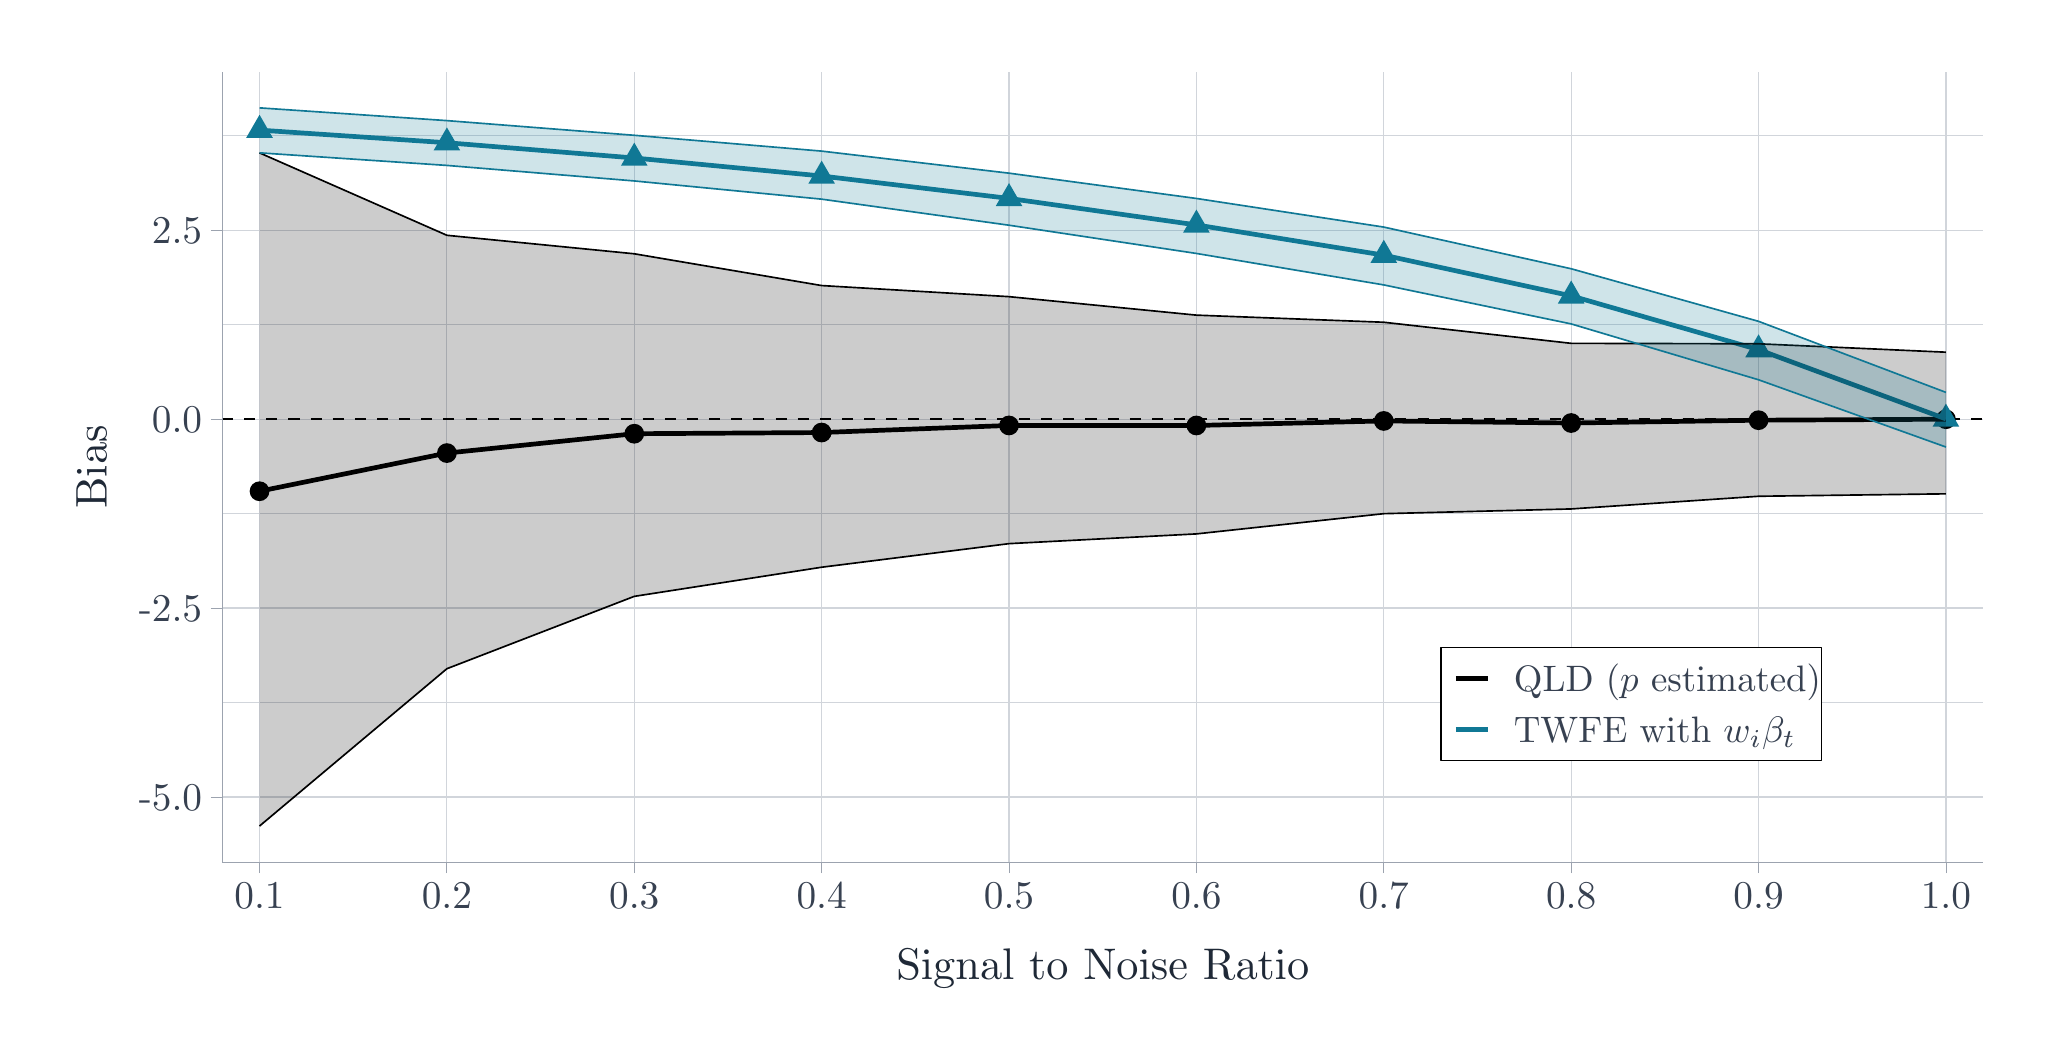
\begin{tikzpicture}[x=1pt,y=1pt]
\definecolor{fillColor}{RGB}{255,255,255}
\path[use as bounding box,fill=fillColor] (0,0) rectangle (722.70,361.35);
\begin{scope}
\path[clip] (  0.00,  0.00) rectangle (722.70,361.35);
\definecolor{drawColor}{RGB}{255,255,255}

\path[draw=drawColor,line width= 0.8pt,line join=round,line cap=round,fill=fillColor] (  0.00,  0.00) rectangle (722.70,361.35);
\end{scope}
\begin{scope}
\path[clip] ( 70.23, 59.89) rectangle (706.70,345.35);
\definecolor{drawColor}{RGB}{255,255,255}
\definecolor{fillColor}{RGB}{255,255,255}

\path[draw=drawColor,line width= 0.8pt,line join=round,line cap=round,fill=fillColor] ( 70.23, 59.89) rectangle (706.70,345.35);
\definecolor{drawColor}{RGB}{209,213,219}

\path[draw=drawColor,line width= 0.4pt,line join=round] ( 70.23,117.50) --
	(706.70,117.50);

\path[draw=drawColor,line width= 0.4pt,line join=round] ( 70.23,185.77) --
	(706.70,185.77);

\path[draw=drawColor,line width= 0.4pt,line join=round] ( 70.23,254.04) --
	(706.70,254.04);

\path[draw=drawColor,line width= 0.4pt,line join=round] ( 70.23,322.31) --
	(706.70,322.31);

\path[draw=drawColor,line width= 0.4pt,line join=round] ( 70.23, 83.36) --
	(706.70, 83.36);

\path[draw=drawColor,line width= 0.4pt,line join=round] ( 70.23,151.63) --
	(706.70,151.63);

\path[draw=drawColor,line width= 0.4pt,line join=round] ( 70.23,219.90) --
	(706.70,219.90);

\path[draw=drawColor,line width= 0.4pt,line join=round] ( 70.23,288.17) --
	(706.70,288.17);

\path[draw=drawColor,line width= 0.4pt,line join=round] ( 83.78, 59.89) --
	( 83.78,345.35);

\path[draw=drawColor,line width= 0.4pt,line join=round] (151.49, 59.89) --
	(151.49,345.35);

\path[draw=drawColor,line width= 0.4pt,line join=round] (219.19, 59.89) --
	(219.19,345.35);

\path[draw=drawColor,line width= 0.4pt,line join=round] (286.90, 59.89) --
	(286.90,345.35);

\path[draw=drawColor,line width= 0.4pt,line join=round] (354.61, 59.89) --
	(354.61,345.35);

\path[draw=drawColor,line width= 0.4pt,line join=round] (422.32, 59.89) --
	(422.32,345.35);

\path[draw=drawColor,line width= 0.4pt,line join=round] (490.03, 59.89) --
	(490.03,345.35);

\path[draw=drawColor,line width= 0.4pt,line join=round] (557.74, 59.89) --
	(557.74,345.35);

\path[draw=drawColor,line width= 0.4pt,line join=round] (625.45, 59.89) --
	(625.45,345.35);

\path[draw=drawColor,line width= 0.4pt,line join=round] (693.16, 59.89) --
	(693.16,345.35);
\definecolor{drawColor}{RGB}{0,0,0}

\path[draw=drawColor,line width= 0.6pt,dash pattern=on 4pt off 4pt ,line join=round] ( 70.23,219.90) -- (706.70,219.90);
\definecolor{fillColor}{RGB}{0,0,0}

\path[fill=fillColor] ( 83.78,193.84) circle (  3.57);

\path[fill=fillColor] (151.49,207.63) circle (  3.57);

\path[fill=fillColor] (219.19,214.62) circle (  3.57);

\path[fill=fillColor] (286.90,215.05) circle (  3.57);

\path[fill=fillColor] (354.61,217.61) circle (  3.57);

\path[fill=fillColor] (422.32,217.60) circle (  3.57);

\path[fill=fillColor] (490.03,219.24) circle (  3.57);

\path[fill=fillColor] (557.74,218.49) circle (  3.57);

\path[fill=fillColor] (625.45,219.51) circle (  3.57);

\path[fill=fillColor] (693.16,219.86) circle (  3.57);
\definecolor{fillColor}{RGB}{16,120,149}

\path[fill=fillColor] ( 83.78,329.88) --
	( 88.58,321.56) --
	( 78.97,321.56) --
	cycle;

\path[fill=fillColor] (151.49,325.32) --
	(156.29,316.99) --
	(146.68,316.99) --
	cycle;

\path[fill=fillColor] (219.19,319.81) --
	(224.00,311.49) --
	(214.39,311.49) --
	cycle;

\path[fill=fillColor] (286.90,313.30) --
	(291.71,304.98) --
	(282.10,304.98) --
	cycle;

\path[fill=fillColor] (354.61,305.20) --
	(359.42,296.88) --
	(349.81,296.88) --
	cycle;

\path[fill=fillColor] (422.32,295.62) --
	(427.13,287.30) --
	(417.52,287.30) --
	cycle;

\path[fill=fillColor] (490.03,284.70) --
	(494.84,276.37) --
	(485.22,276.37) --
	cycle;

\path[fill=fillColor] (557.74,269.99) --
	(562.55,261.67) --
	(552.93,261.67) --
	cycle;

\path[fill=fillColor] (625.45,250.54) --
	(630.26,242.22) --
	(620.64,242.22) --
	cycle;

\path[fill=fillColor] (693.16,225.51) --
	(697.96,217.19) --
	(688.35,217.19) --
	cycle;

\path[draw=drawColor,line width= 1.7pt,line join=round] ( 83.78,193.84) --
	(151.49,207.63) --
	(219.19,214.62) --
	(286.90,215.05) --
	(354.61,217.61) --
	(422.32,217.60) --
	(490.03,219.24) --
	(557.74,218.49) --
	(625.45,219.51) --
	(693.16,219.86);
\definecolor{drawColor}{RGB}{16,120,149}

\path[draw=drawColor,line width= 1.7pt,line join=round] ( 83.78,324.33) --
	(151.49,319.77) --
	(219.19,314.26) --
	(286.90,307.75) --
	(354.61,299.65) --
	(422.32,290.07) --
	(490.03,279.15) --
	(557.74,264.44) --
	(625.45,244.99) --
	(693.16,219.96);
\definecolor{fillColor}{RGB}{0,0,0}

\path[fill=fillColor,fill opacity=0.20] ( 83.78,316.11) --
	(151.49,286.32) --
	(219.19,279.64) --
	(286.90,268.16) --
	(354.61,264.15) --
	(422.32,257.47) --
	(490.03,254.90) --
	(557.74,247.28) --
	(625.45,247.12) --
	(693.16,244.08) --
	(693.16,192.90) --
	(625.45,192.02) --
	(557.74,187.44) --
	(490.03,185.73) --
	(422.32,178.42) --
	(354.61,174.90) --
	(286.90,166.38) --
	(219.19,155.85) --
	(151.49,129.71) --
	( 83.78, 72.86) --
	cycle;
\definecolor{drawColor}{RGB}{0,0,0}

\path[draw=drawColor,line width= 0.6pt,line join=round] ( 83.78,316.11) --
	(151.49,286.32) --
	(219.19,279.64) --
	(286.90,268.16) --
	(354.61,264.15) --
	(422.32,257.47) --
	(490.03,254.90) --
	(557.74,247.28) --
	(625.45,247.12) --
	(693.16,244.08);

\path[draw=drawColor,line width= 0.6pt,line join=round] (693.16,192.90) --
	(625.45,192.02) --
	(557.74,187.44) --
	(490.03,185.73) --
	(422.32,178.42) --
	(354.61,174.90) --
	(286.90,166.38) --
	(219.19,155.85) --
	(151.49,129.71) --
	( 83.78, 72.86);
\definecolor{fillColor}{RGB}{16,120,149}

\path[fill=fillColor,fill opacity=0.20] ( 83.78,332.37) --
	(151.49,327.76) --
	(219.19,322.46) --
	(286.90,316.74) --
	(354.61,308.77) --
	(422.32,299.63) --
	(490.03,289.29) --
	(557.74,274.23) --
	(625.45,255.23) --
	(693.16,229.56) --
	(693.16,209.81) --
	(625.45,234.11) --
	(557.74,254.30) --
	(490.03,268.39) --
	(422.32,279.76) --
	(354.61,289.96) --
	(286.90,299.38) --
	(219.19,305.96) --
	(151.49,311.57) --
	( 83.78,316.12) --
	cycle;
\definecolor{drawColor}{RGB}{16,120,149}

\path[draw=drawColor,line width= 0.6pt,line join=round] ( 83.78,332.37) --
	(151.49,327.76) --
	(219.19,322.46) --
	(286.90,316.74) --
	(354.61,308.77) --
	(422.32,299.63) --
	(490.03,289.29) --
	(557.74,274.23) --
	(625.45,255.23) --
	(693.16,229.56);

\path[draw=drawColor,line width= 0.6pt,line join=round] (693.16,209.81) --
	(625.45,234.11) --
	(557.74,254.30) --
	(490.03,268.39) --
	(422.32,279.76) --
	(354.61,289.96) --
	(286.90,299.38) --
	(219.19,305.96) --
	(151.49,311.57) --
	( 83.78,316.12);
\end{scope}
\begin{scope}
\path[clip] (  0.00,  0.00) rectangle (722.70,361.35);
\definecolor{drawColor}{RGB}{156,163,175}

\path[draw=drawColor,line width= 0.3pt,line join=round] ( 70.23, 59.89) --
	( 70.23,345.35);
\end{scope}
\begin{scope}
\path[clip] (  0.00,  0.00) rectangle (722.70,361.35);
\definecolor{drawColor}{RGB}{55,65,81}

\node[text=drawColor,anchor=base east,inner sep=0pt, outer sep=0pt, scale=  1.42] at ( 63.03, 78.46) {-5.0};

\node[text=drawColor,anchor=base east,inner sep=0pt, outer sep=0pt, scale=  1.42] at ( 63.03,146.73) {-2.5};

\node[text=drawColor,anchor=base east,inner sep=0pt, outer sep=0pt, scale=  1.42] at ( 63.03,215.00) {0.0};

\node[text=drawColor,anchor=base east,inner sep=0pt, outer sep=0pt, scale=  1.42] at ( 63.03,283.28) {2.5};
\end{scope}
\begin{scope}
\path[clip] (  0.00,  0.00) rectangle (722.70,361.35);
\definecolor{drawColor}{RGB}{156,163,175}

\path[draw=drawColor,line width= 0.3pt,line join=round] ( 66.23, 83.36) --
	( 70.23, 83.36);

\path[draw=drawColor,line width= 0.3pt,line join=round] ( 66.23,151.63) --
	( 70.23,151.63);

\path[draw=drawColor,line width= 0.3pt,line join=round] ( 66.23,219.90) --
	( 70.23,219.90);

\path[draw=drawColor,line width= 0.3pt,line join=round] ( 66.23,288.17) --
	( 70.23,288.17);
\end{scope}
\begin{scope}
\path[clip] (  0.00,  0.00) rectangle (722.70,361.35);
\definecolor{drawColor}{RGB}{156,163,175}

\path[draw=drawColor,line width= 0.3pt,line join=round] ( 70.23, 59.89) --
	(706.70, 59.89);
\end{scope}
\begin{scope}
\path[clip] (  0.00,  0.00) rectangle (722.70,361.35);
\definecolor{drawColor}{RGB}{156,163,175}

\path[draw=drawColor,line width= 0.3pt,line join=round] ( 83.78, 55.89) --
	( 83.78, 59.89);

\path[draw=drawColor,line width= 0.3pt,line join=round] (151.49, 55.89) --
	(151.49, 59.89);

\path[draw=drawColor,line width= 0.3pt,line join=round] (219.19, 55.89) --
	(219.19, 59.89);

\path[draw=drawColor,line width= 0.3pt,line join=round] (286.90, 55.89) --
	(286.90, 59.89);

\path[draw=drawColor,line width= 0.3pt,line join=round] (354.61, 55.89) --
	(354.61, 59.89);

\path[draw=drawColor,line width= 0.3pt,line join=round] (422.32, 55.89) --
	(422.32, 59.89);

\path[draw=drawColor,line width= 0.3pt,line join=round] (490.03, 55.89) --
	(490.03, 59.89);

\path[draw=drawColor,line width= 0.3pt,line join=round] (557.74, 55.89) --
	(557.74, 59.89);

\path[draw=drawColor,line width= 0.3pt,line join=round] (625.45, 55.89) --
	(625.45, 59.89);

\path[draw=drawColor,line width= 0.3pt,line join=round] (693.16, 55.89) --
	(693.16, 59.89);
\end{scope}
\begin{scope}
\path[clip] (  0.00,  0.00) rectangle (722.70,361.35);
\definecolor{drawColor}{RGB}{55,65,81}

\node[text=drawColor,anchor=base,inner sep=0pt, outer sep=0pt, scale=  1.42] at ( 83.78, 42.89) {0.1};

\node[text=drawColor,anchor=base,inner sep=0pt, outer sep=0pt, scale=  1.42] at (151.49, 42.89) {0.2};

\node[text=drawColor,anchor=base,inner sep=0pt, outer sep=0pt, scale=  1.42] at (219.19, 42.89) {0.3};

\node[text=drawColor,anchor=base,inner sep=0pt, outer sep=0pt, scale=  1.42] at (286.90, 42.89) {0.4};

\node[text=drawColor,anchor=base,inner sep=0pt, outer sep=0pt, scale=  1.42] at (354.61, 42.89) {0.5};

\node[text=drawColor,anchor=base,inner sep=0pt, outer sep=0pt, scale=  1.42] at (422.32, 42.89) {0.6};

\node[text=drawColor,anchor=base,inner sep=0pt, outer sep=0pt, scale=  1.42] at (490.03, 42.89) {0.7};

\node[text=drawColor,anchor=base,inner sep=0pt, outer sep=0pt, scale=  1.42] at (557.74, 42.89) {0.8};

\node[text=drawColor,anchor=base,inner sep=0pt, outer sep=0pt, scale=  1.42] at (625.45, 42.89) {0.9};

\node[text=drawColor,anchor=base,inner sep=0pt, outer sep=0pt, scale=  1.42] at (693.16, 42.89) {1.0};
\end{scope}
\begin{scope}
\path[clip] (  0.00,  0.00) rectangle (722.70,361.35);
\definecolor{drawColor}{RGB}{31,41,55}

\node[text=drawColor,anchor=base,inner sep=0pt, outer sep=0pt, scale=  1.60] at (388.47, 17.56) {Signal to Noise Ratio};
\end{scope}
\begin{scope}
\path[clip] (  0.00,  0.00) rectangle (722.70,361.35);
\definecolor{drawColor}{RGB}{31,41,55}

\node[text=drawColor,rotate= 90.00,anchor=base,inner sep=0pt, outer sep=0pt, scale=  1.60] at ( 28.57,202.62) {Bias};
\end{scope}
\begin{scope}
\path[clip] (  0.00,  0.00) rectangle (722.70,361.35);
\definecolor{drawColor}{RGB}{0,0,0}
\definecolor{fillColor}{RGB}{255,255,255}

\path[draw=drawColor,line width= 0.6pt,line join=round,line cap=round,fill=fillColor] (510.59, 96.53) rectangle (648.22,137.43);
\end{scope}
\begin{scope}
\path[clip] (  0.00,  0.00) rectangle (722.70,361.35);
\definecolor{drawColor}{RGB}{255,255,255}
\definecolor{fillColor}{RGB}{255,255,255}

\path[draw=drawColor,line width= 0.8pt,line join=round,line cap=round,fill=fillColor] (514.59,118.98) rectangle (529.05,133.43);
\end{scope}
\begin{scope}
\path[clip] (  0.00,  0.00) rectangle (722.70,361.35);
\definecolor{fillColor}{RGB}{0,0,0}

\path[fill=fillColor] (521.82,126.21) circle (  0.36);
\end{scope}
\begin{scope}
\path[clip] (  0.00,  0.00) rectangle (722.70,361.35);
\definecolor{drawColor}{RGB}{0,0,0}

\path[draw=drawColor,line width= 1.7pt,line join=round] (516.04,126.21) -- (527.60,126.21);
\end{scope}
\begin{scope}
\path[clip] (  0.00,  0.00) rectangle (722.70,361.35);
\definecolor{drawColor}{RGB}{255,255,255}
\definecolor{fillColor}{RGB}{255,255,255}

\path[draw=drawColor,line width= 0.8pt,line join=round,line cap=round,fill=fillColor] (514.59,100.53) rectangle (529.05,114.98);
\end{scope}
\begin{scope}
\path[clip] (  0.00,  0.00) rectangle (722.70,361.35);
\definecolor{fillColor}{RGB}{16,120,149}

\path[fill=fillColor] (521.82,108.31) --
	(522.30,107.48) --
	(521.34,107.48) --
	cycle;
\end{scope}
\begin{scope}
\path[clip] (  0.00,  0.00) rectangle (722.70,361.35);
\definecolor{drawColor}{RGB}{16,120,149}

\path[draw=drawColor,line width= 1.7pt,line join=round] (516.04,107.75) -- (527.60,107.75);
\end{scope}
\begin{scope}
\path[clip] (  0.00,  0.00) rectangle (722.70,361.35);
\definecolor{drawColor}{RGB}{55,65,81}

\node[text=drawColor,anchor=base west,inner sep=0pt, outer sep=0pt, scale=  1.33] at (537.05,121.62) {QLD ($p$ estimated)};
\end{scope}
\begin{scope}
\path[clip] (  0.00,  0.00) rectangle (722.70,361.35);
\definecolor{drawColor}{RGB}{55,65,81}

\node[text=drawColor,anchor=base west,inner sep=0pt, outer sep=0pt, scale=  1.33] at (537.05,103.16) {TWFE with $\bm{w}_i \beta_t$};
\end{scope}
\end{tikzpicture}
